\documentclass[12pt,titlepage,a4page , tikz , multi,table , svgnames,xcdraw]{article}
\usepackage{graphicx}
\usepackage[svgnames , table , xcdraw]{xcolor}
\usepackage{fancyhdr}
\usepackage{fixltx2e}

\usepackage{hyperref}
\hypersetup{
    colorlinks=true,
    linkcolor=blue,
    filecolor=magenta,
    urlcolor=cyan,
}

\usepackage{mathtools}
\usepackage{multirow}
\usepackage{graphicx}
\usepackage[ruled,vlined]{algorithm2e}
\usepackage{float}
\usepackage{enumitem}
\usepackage{listings }
\usepackage[a4paper, total={6in, 8in}]{geometry}
\usepackage{afterpage}
\usepackage{amssymb}
\usepackage{pdflscape}
\usepackage{lscape}
\usepackage{amsmath}
\usepackage{svg}
\usepackage[final]{pdfpages}
\usepackage{pgf, tikz}
\usetikzlibrary{arrows, automata}
\usetikzlibrary{shapes.multipart}


\DeclareMathOperator\arctanh{arctanh}

\usepackage[T1]{fontenc}
\usepackage{tikz}
\usepackage[utf8]{inputenc} % Required for inputting international characters
\usepackage{PTSerif}

\usepackage{float}

\usepackage[Kashida]{xepersian}
\settextfont[
 BoldFont={XB Zar bold.ttf}
 ]{XB Zar.ttf}


\NewDocumentCommand{\codeword}{v}{
\texttt{\textcolor{blue}{#1}}
}
\DeclareFixedFont{\ttb}{T1}{txtt}{bx}{n}{12} % for bold
\DeclareFixedFont{\ttm}{T1}{txtt}{m}{n}{12}  % for normal


\definecolor{deepblue}{rgb}{0,0,0.5}
\definecolor{deepred}{rgb}{0.6,0,0}
\definecolor{deepgreen}{rgb}{0,0.5,0}

\hypersetup{citecolor=blue}

\newcommand\independent{\protect\mathpalette{\protect\independenT}{\perp}}
\def\independenT#1#2{\mathrel{\rlap{$#1#2$}\mkern2mu{#1#2}}}

% Python style for highlighting
\newcommand\pythonstyle{\lstset{
language=Python,
basicstyle=\ttm,
otherkeywords={self},             % Add keywords here
keywordstyle=\ttb\color{deepblue},
emph={MyClass,__init__},          % Custom highlighting
emphstyle=\ttb\color{deepred},    % Custom highlighting style
stringstyle=\color{deepgreen},
frame=tb,                         % Any extra options here
showstringspaces=false            %
}}


% Python environment
\lstnewenvironment{python}[1][]
{
\pythonstyle
\lstset{#1}
}
{}

% Python for external files
\newcommand\pythonexternal[2][]{{
\pythonstyle
\lstinputlisting[#1]{#2}}}

\newenvironment{changemargin}[2]{%
\begin{list}{}{%
\setlength{\topsep}{0pt}%
\setlength{\leftmargin}{#1}%
\setlength{\rightmargin}{#2}%
\setlength{\listparindent}{\parindent}%
\setlength{\itemindent}{\parindent}%
\setlength{\parsep}{\parskip}%
}%
\item[]}{\end{list}}

% Python for inline
\newcommand\pythoninline[1]{{\pythonstyle\lstinline!#1!}}


\begin{document}

\begin{titlepage}

 \begin{center}

       \vspace*{0.5cm}

 \vspace{0.5cm}
       \textbf{ \Huge{به نام خدا} }
       \vspace{0.2cm}

       
\includegraphics[width=0.4\textwidth]{Images/sharif.png}

 	\vspace{0.3cm}
       \textbf{ \LARGE{تحلیل و طراحی سیستم‌ها} }


   \vspace{0.3cm}
  \textbf{ \Large{سامانه مشاوره آنلاین} }
   \vspace{0.3cm}


      \large \textbf{دانشکده مهندسی کامپیوتر}\\\vspace{0.2cm}
    \large   دانشگاه صنعتی شریف\\\vspace{0.25cm}

% استاد:\\
    \vspace{0.15cm}
    \noindent\rule[1ex]{\linewidth}{3pt}

    \vspace{0.5cm}
نام، نام خانوادگی و شماره دانشجویی اعضای گروه:\\


        \textbf{{فرزام زهدی‌نسب - 97105996}}
        \vspace{0.05cm}

        \textbf{{یاشار ظروفچی - 97106119}}
        \vspace{0.05cm}

        \textbf{{علی بالاپور - 97101326}}
        \vspace{0.05cm}
        

\end{center}
\end{titlepage}

\newpage
\pagestyle{fancy}
\fancyhf{}
\fancyfoot{}

\cfoot{\thepage}
\chead{سامانه مشاوره آنلاین}
\rhead{پیشنهادنامه}
\lhead{تحلیل و طراحی سیستم‌ها}

\tableofcontents

\newpage


\section{اهداف پروژه}

\subsection{مقدمه}
با پیشرفت تکنولوژی و افزایش ضریب نفوذ رایانه و اینترنت در زندگی روزمره، پتانسیل ایجاد تغییر در برخی از کارهای روزمره انسان به وجود آمده است. اعضای جامعه ما برای انجام بسیاری از کارها (مانند پرداخت قبض، شرکت در کلاس‌های آموزشی و ...) در گذشته می‌بایست به مکان‌های خاصی مراجعه می‌کردند و بعضاً بخش عظیمی از زمان خود را در صف و در انتظار می‌گذراند. اما با افزایش امکانات و خدمات اینترنت، بسیاری از این اتلاف وقت‌ها کاهش یافته و امروزه می‌توان با استفاده از اینترنت و تنها با چند کلیک، بسیاری از کارهای زمان‌بر را به‌راحتی انجام داد. \\
البته لازم به ذکر است که این تغییر در برخی از حوزه‌ها، مانند مراجعه به پزشک و مشاور، به‌طور کامل جا نیافتاده است و اکثر افراد امروزه تمایل به مراجعه حضوری برای معاینات پزشکی و مشاوره را دارند. در سالیان اخیر و با معرفی چندین سرویس در این حوزه (مانند اسنپ و زوپ) و همچنین بیماری کرونا و ایجاد محدودیت‌های مربوط به پروتکل‌ها، این موضوع نیز در حال تغییر می‌باشد اما هنوز هم تعداد و کیفیت این سرویس‌ها جای پیشرفت دارد. \\
برای همین در این پروژه قصد داریم تا یک سامانه اختصاصی برای مشاوره روانشناسی و پزشکی طراحی و پیاده‌سازی کنیم که در آن مشاوران، روانشناسان، روان‌پزشکان، و پزشکان حاذق به ارائه خدمات به متقاضیان مشاوره بپردازند. 

\subsection{اهداف کلی}
یکی از اهداف اصلی این سامانه، راحت‌تر کردن ایجاد ارتباط میان کاربر و مشاور مناسب است. به‌طور سنتی، هر فرد با توجه به محل زندگی، انتخاب محدودی بین مشاوران مدنظر داشت و برای گرفتن وقت مشاوره می‌بایست از همان تعداد محدود فردی را به‌عنوان مشاور انتخاب می‌کرد. در شهرهای کوچک و کم برخوردار نیز معمولاً مشاور و پزشکان مطرح زیادی وجود ندارند و این موضوع باعث به وجود آمدن نوعی بی‌عدالتی در حق ساکنان این نوع شهرها می‌شود. با استفاده از این سامانه، این مشکل به‌طور کامل حل می‌شود. کاربران می‌توانند با استفاده از این سامانه و با فیلتر کردن انتخاب‌های خود، بهترین مشاور را انتخاب کنند. \\
هدف دیگر سامانه کاهش اتلاف زمان، انرژی و هزینه جهت مراجعه حضوری برای مشاوره می‌باشد. با استفاده از این سامانه، فرآیند مشاوره به‌طور کامل به‌صورت مجازی (با استفاده از چت باکس و یا به‌صورت ویدیویی) انجام می‌شود و کاربر لازم نیست که به‌صورت حضوری به مطب مشاور مراجعه کند. این کار، علاوه بر کاهش هزینه‌های رفت آمد، منجر به کاهش ترافیک و مصرف سوخت نیز می‌گردد. همچنین کاربر لازم نیست مدت‌زمان طولانی‌ای را برای رسیدن به مطب مشاوره صرف نماید. این سامانه به مشاوران نیز کمک می‌کند تا بتوانند از زمان اضافه خود استفاده بهینه داشته باشند. \\
هدف دیگر این سامانه ایجاد نوعی رقابت سالم میان مشاوران برای ارتقای سطح خدمات مشاوره می‌باشد. برای این منظور یک سیستم امتیازدهی دقیق برای هر جلسه مشاوره تدارک دیده خواهد شد تا یک معیار سنجش برای هر مشاور ایجاد شود و این منجر به ایجاد نوعی رقابت بین مشاوران برای ارتقای سطح عملکرد خود خواهد شد. 

\subsection{خلاصه اهداف}
\begin{itemize}
\item تحلیل، طراحی و پیاده‌سازی سامانه مشاوره آنلاین
\item ایجاد امکان دریافت مشاوره برای همه ساکنین ایران
\item ایجاد امکان عضویت مشاوران سرتاسر کشور برای شناساندن بیشتر خود
\item کاهش اتلاف وقت و هزینه صرف‌شده جهت مراجعه حضوری برای مشاوره
\item ایجاد فضای رقابت سالم میان مشاوران جهت بهبود عملکرد با استفاده از سیستم امتیازدهی
\end{itemize}

\newpage

\section{پیش‌زمینه پروژه}
\subsection{عوامل طرح مسئله}
سه عامل اصلی شروع یک پروژه تحلیل، طراحی و پیاده‌سازی سیستم اطلاعاتی موارد زیر می‌توانند ‌باشند:
\begin{itemize}
\item مشکل یا مسئله (Problem)ای که یک نیاز را بوجود می‌آورد.
\item فرصت (Opportunity) برای بهبود عملکرد
\item دستور از مراجع بالا (Directive) برای ایجاد تغییرات
\end{itemize}
دو عامل اصلی این پروژه، از جنس مشکل و فرصت می‌باشد. مشکل و مسئله این است که با توجه به حضور متمرکز اکثر مشاوران و متخصصان مطرح در شهرهای بزرگ، دسترسی نداشتن آحاد مردم به مشاوران مناسب، اتلاف وقت و هزینه جهت مراجعه حضوری، و همچنین در دسترس نبودن مشاور در هر زمان وجود چنین سامانه‌ای در سطح کشور احساس می‌شود. از طرفی با توجه به گسترش بیماری کرونا و نبود بستر مناسب جهت مشاوره آنلاین، این فرصت به وجود آمده تا یک سامانه مشاوره آنلاین بتواند عملکرد مناسبی داشته باشد. در این بخش به بررسی بیشتر این مشکل و فرصت می‌پردازیم.


\subsection{مشکل}
همان‌گونه که در بخش‌های قبلی اشاره شد، مشکل دسترسی نداشتن ساکنان شهرهای کم برخوردار به مشاوران مجرب و همچنین اتلاف وقت و هزینه برای حضور در مطب مشاوره، یکی از عوامل ایجاد سامانه مشاوره آنلاین است. با راه‌اندازی این سامانه، افراد خواهان مشاوره صرفاً با یک ثبت‌نام و یک جستجوی ساده، مشاور موردنظر خود را پیدا می‌کنند و حتی در صورت نیافتن مشاور مدنظر، با استفاده از سیستم جستجوی پیشرفته و یا سیستم توصیه‌گر مشاور مناسب را می‌یابند. همچنین با توجه به آنلاین بودن سامانه و قرار مشاوره، افراد می‌توانند در اکثر ساعات روز، از خدمات مشاوره بهره‌مند شوند. همچنین ساکنان شهرهای کوچک و کم برخوردار نیز از امکان مشاوره با متخصصان مجرب برخوردار می‌گردند. این سامانه می‌تواند از اتلاف وقت و هزینه برای رفت‌وآمد به مطب مشاوره را بکاهد و تأثیری (هرچند اندک) بر روی کاهش استفاده از وسایل نقلیه و ترافیک بگذارد.

\subsection{فرصت}
با شروع همه‌گیری بیماری کرونا، یک فرصت برای کسب‌وکارها در اکثر زمینه‌ها (آموزش، خدمات و ...) فراهم گردید تا با ایجاد بستر آنلاین برای ارائه خدمات، کسب‌وکار خود را گسترش دهند. برای مثال دانشگاه شریف قصد ایجاد یک بستر آنلاین برای ارائه درس‌ها و آموزش‌های خود داشت اما این پروژه قبل از دوران همه‌گیری، به‌کندی پیش می‌رفت. با شروع همه‌گیری، این پروژه با سرعت بیشتری پیگیری شد و اکنون اکثر دروس دانشگاه در این بستر ارائه می‌شود. \\
با توجه به فرصت پیش‌آمده، می‌توان با ارائه یک سامانه و سرویس اختصاصی مشاوره آنلاین، هم به نیاز به وجود آمده پاسخ مناسب داد و ازنظر مالی و اقتصادی، عملکرد مناسبی داشت.




\newpage


\section{گستره‌ی پروژه}
\subsection{ذینفعان سامانه}
\subsubsection{مالکین}
مالک این پروژه جناب آقای دکتر حیدرنوری، استاد درس تحلیل و طراحی سیستم‌ها، می‌باشد. 

\subsubsection{کاربران}
سه دسته کاربران سامانه را تشکیل می‌دهند:
\begin{itemize}
\item متقاضیان مشاوره: افرادی که می‌خواهند از خدمات مشاوره آنلاین (چه به‌صورت متنی و چه به‌صورت ویدیویی) استفاده نمایند. آن‌ها می‌توانند با استفاده از سیستم جستجو (ساده و پیشرفته) و لیست مشاوران، مشاور مناسب خود را پیدا کرده و درخواست وقت مشاوره بنمایند.
\item مشاوران: این افراد متخصصان مشاوره در زمینه روانشناسی و پزشکی و ... هستند. این کاربران زمان حضور خود جهت مشاوره را مشخص می‌نمایند و در صورت تأیید، به فرد متقاضی به‌صورت متنی یا ویدیویی، مشاوره می‌دهند. 
\item مدیران سامانه: این افراد به مدیریت سامانه و بررسی صلاحیت مشاوران بر اساس مدارک ارسالی آن‌ها می‌پردازند. همچنین این افراد بر کاربران نظارت دارند.
\end{itemize}
\subsubsection{تحلیلگران و طراحان سامانه}

\subsubsection{مدیر پروژه}

\subsubsection{فراهم‌کنندگان سرویس خارجی}
در این پروژه از پلتفرم \href{https://meet.jit.si/}{jitsi} برای تهیه بستر ملاقات ویدیوی استفاده خواهد شد.

\subsection{داده‌ها}
داده‌های زیر در این سامانه ذخیره می‌گردند:

\subsubsection{اطلاعات کاربران}
		همه کاربران در این سامانه دارای پروفایل هستند. در پروفایل کاربران عادی یا متقاضیان مشاوره، اطلاعاتی مانند نام، نام خانوادگی، جنسیت، شماره تلفن، سال تولد ذخیره می‌شود. در پروفایل مشاوران، اطلاعاتی مانند نام، نام خانوادگی، جنسیت، حوزه‌های تخصص، اطلاعات مربوط به مدرک، شماره عضویت در نظام پزشکی، شماره تماس، آدرس مطب (در صورت وجود) ذخیره می‌گردد.
همچنین امتیازاتی که هر کاربر به هر مشاور (پس از مشاوره) داده است نیز ذخیره می‌گردند. البته این اطلاعات به‌گونه‌ای ذخیره خواهند شد که حریم شخصی هر کاربر حفظ شود.

\subsubsection{اطلاعات جلسه مشاوره}
اطلاعات مربوط به هر جلسه مشاوره مانند مدت زمان، تاریخ، نام مشاور و کاربر عادی، موضوع مشاوره و تراکنش بانکی انجام شده مربوط به این جلسه ذخیره می‌گردند.

\subsubsection{تراکنش‌ها}
همه تراکنش‌های مربوط به سامانه مانند جستجوها، بازدید از پروفایل مشاوران، همه پرسش‌های کاربران و سایر تراکنش‌ها ذخیره می‌گردند.

\subsection{امکانات}
\subsubsection{امکانات مربوط به متقاضیان مشاوره}
\begin{itemize}
    \item امکان ایجاد حساب کاربری با ثبت اطلاعات مورد نیاز (نام، نام خانوادگی، شماره‌ تلفن، رمز عبور و ...)
	\item امکان تعریف مشکلات و سابقه بیماری
	\item امکان جستجوی مشاور بر اساس حوزه کاری و همچنین امکان استفاده از سیستم جستجوی پیشرفته
	\item امکان مشاوره با مشاوران سراسر ایران (در صورت حضور مشاور در سامانه) به صورت متنی (از طریق پیامرسان داخل سامانه) و ویدیویی (از طریق پلتفرم‌های ارتباط ویدیویی مانند jitsi) بهمراه ارسال توضیحات قبل از مشاوره
	\item امکان مشاهده زمان‌های در دسترس بودن هر مشاور به‌همراه هزینه ویزیت
	\item امکان امتیازدهی و نظردهی به هر مشاور پس از مشاوره
	\item امکان کنسل کردن زمان مشاوره 24 ساعت قبل از زمان جلسه مشاوره و مسترد شدن بخشی از مبلغ 
	\item امکان مشاهده لیست مشاوران بر اساس تخصص و امتیاز کسب‌شده
	\item امکان تهیه لیست مشاوران مورد علاقه 
    \item امکان مشاهده نوبت‌های کاربر، اطلاعات مربوط به مشاوره‌های قبلی، میزان شارژ حساب کاربری، تراکنش‌های انجام‌شده
\end{itemize}

\subsubsection{امکانات مربوط به مشاوران}
\begin{itemize}
    \item امکان ثبت‌نام با ثبت مدارک موردنیاز (نام و نام خانوادگی، کد ملی، مجوز طبابت، مدرک تحصیلی، شماره تماس و ...) و تایید مدیران سایت
	\item امکان مشاوره‌دادن به کاربران متقاضی مشاوره
	\item امکان تعیین بهای ویزیت و زمان‌های دردسترس برای مشاوره
	\item امکان مشاهده لیست جلسات مشاوره آتی
	\item امکان کنسل کردن زمان مشاوره 24 ساعت قبل از زمان مشاوره (و مسترد شدن هزینه به کاربر)
	\item امکان مشاهده سوابق مشاوره و مشکلات فردی هر فرد متقاضی مشاوره
	\item امکان گزارش کاربران متخلف به مدیران
	\item امکان مشاهده اطلاعات مربوط مشاوره‌های قبلی، میزان شارژ حساب کاربری، تراکنش‌های انجام شده
\end{itemize}

\subsubsection{امکانات مربوط به مدیران سامانه}
\begin{itemize}
\item امکان تایید ثبت‌نام مشاوران و پزشکان با توجه به مدارک ارسال‌شده
\item امکان حذف کاربران متخلف
\end{itemize}
\subsubsection{امکانات مازاد (backlog)}
در صورت داشتن زمان یا بودجه اضافی، می توان این موارد را نیز در سیستم پیاده‌سازی کرد:
\begin{itemize}
\item سیستم توصیه‌گر مشاور (بر اساس مشاوره‌ها، امتیاز ثبت‌شده توسط کاربر برای هر مشاوره، و همچنین مشکلات ثبت شده بیمار)
\item پیاده‌سازی بخش پرسش و پاسخ رایگان: در این بخش بیماران می‌توانند سوالات کلی خود را بپرسند و پزشکان و مشاوران به این سوالات پاسخ دهند. هر کدام از بیماران محدودیتی در تعداد ارسال سوالات دارند و همچنین برای هر پزشک پاسخ‌دهنده، امتیاز مثبت ثبت می‌گردد.
\end{itemize}

\subsection{گستره مکانی}
همه مشاوران متخصص در سرتاسر ایران توانایی عضویت در این سامانه و مشاوره‌دادن به کاربران را دارند. همچنین همه افراد نیز می‌‌توانند از خدمات مشاوره این سامانه استفاده نمایند.

\newpage
\section{رویکرد پروژه}
رویکرد پروژه به صورت محصول‌محور خواهد بود و از روش توسعه چابک نرم‌افزار استفاده خواهیم کرد. 
این رویکرد مبتنی بر تکرار است و امکانات محصول به تدریج به آن اضافه خواهند شد و پیشرفت محصول قابل لمس و مشاهده خواهد بود. 
این روش برنامه‌ریزی تطبیقی، توسعه، تحویل تکاملی و رویکرد زمان بسته‌بندی تکرارشونده را ارتقا بخشیده و پاسخ‌های سریع و انعطاف‌پذیر برای انجام تغییرات در محصول را تقویت می‌کند.

\subsection{مسیر پروژه}

در فاز صفر، مسئله و گستره‌ی آن را به طور دقیق مشخص می‌کنیم.

در فاز یکم به به تحلیل مسئله
\footnote{\lr{Problem Analysis}}
و بررسی نیازمندی‌ها
\footnote{\lr{Requirements Analysis}}
می‌پردازیم.
سپس با توجه به نیازمندی‌ها و از روی اصول مشخص، نمودار مورد کاربرد را بدست خواهیم آورد. در این فاز باید مکانیزم‌های سامانه به گونه‌ای تعریف شوند که حداکثر رضایت ذی‌النفعان مختلف جلب شود.

در فاز دوم به مدل‌سازی فرآیندها و بانک‌های اطلاعاتی یا به عبارت دیگر، طراحی منطقی
\footnote{\lr{Logical Design}}
می‌پردازیم. در این فاز با استفاده از نیازمندی‌های جمع‌آوری شده به مشخص کردن موجودیت‌ها، صفات و نوع ارتباط میان آن‌ها خواهیم پرداخت. همچنین محدودیت‌های پیاده‌سازی در این فاز مشخص خواهند شد.

در فاز سوم با استفاده از نمودار‌های تولید شده در فاز‌های قبلی به پیاده‌سازی و ارزیابی سامانه اطلاعاتی با بهره گرفتن از شیوه‌ی چابک اسکرام می‌پردازیم.

\newpage
\subsection{تحویل‌دادنی‌ها}
تحویل‌دادنی‌ها (خروجی) هر فاز از پروژه به صورت زیر خواهد بود:

\begin{itemize}
    \item فاز صفر
    
    پیشنهادنامه‌ی پروژه
    \item فاز یکم
    
    نمودار مورد کاربرد
    \footnote{\lr{Use Case}}
    
    سناریوهای سامانه
    \item فاز دوم
    
    نمودار جریان‌داده‌ها
    \footnote{\lr{Data flow Diagram}} 
    (مدل‌سازی فرآیند‌ها)
    
    نمودار داده رابطه‌ای (مدل‌سازی بانک‌های اطلاعاتی)
    \item فاز سوم
    
    نسخه‌نهایی محصول
    
    مستندات پروژه
    
\end{itemize}



\newpage
\section{رهیافت مدیریت}
\subsection{مدیریت، تجارب و وظایف}
\subsubsection{مدیر پروژه}

\resizebox{\columnwidth}{!}{%
\begin{tabular}{|cccc|}
\hline
\multicolumn{4}{|c|}{مدیر پروژه}                                                                                                                                                                                                      \\ \hline
\multicolumn{1}{|c|}{نام و نام‌خانوادگی} & \multicolumn{1}{c|}{مدرک تحصیلی}              & \multicolumn{1}{c|}{سابقه مرتبط} & \multicolumn{1}{c|}{شرح سوابق کاری}                               \\ \hline
\multicolumn{1}{|c|}{یاشار ظروفچی}       & \multicolumn{1}{c|}{کارشناسی مهندسی کامپیوتر} & \multicolumn{1}{c|}{۳ ماه}      & \multicolumn{1}{c|}{تدوینگر برنامه‌ی کارآموزی کد استار بک‌اند و راهبر دوره‌ در تابستان ۱۴۰۰}     \\ \hline
\end{tabular}
}

\subsubsection{اعضا، سوابق و توانمندی‌ها}

\resizebox{\columnwidth}{!}{%
\begin{tabular}{|ccccc|}
\hline
\multicolumn{5}{|c|}{اعضا}                                                                                                                                                                                                           \\ \hline
\multicolumn{1}{|c|}{نام و نام‌خانوادگی} & \multicolumn{1}{c|}{مدرک تحصیلی}              & \multicolumn{1}{c|}{سابقه کاری} & \multicolumn{1}{c|}{شرح سوابق کاری}                         & توانمندی‌ها                               \\ \hline
\multicolumn{1}{|c|}{یاشار ظروفچی}       & \multicolumn{1}{c|}{کارشناسی مهندسی کامپیوتر} & \multicolumn{1}{c|}{۳ سال}      & \multicolumn{1}{c|}{مهندس نرم‌افزار اپلیکیشن بله}           & ‌Backend                                  \\ \hline
\multicolumn{1}{|c|}{علی بالاپور}        & \multicolumn{1}{c|}{کارشناسی مهندسی کامپیوتر} & \multicolumn{1}{c|}{۲ ماه}      & \multicolumn{1}{c|}{تجربه کار با adobe XD برای طراحی UI/UX} & adobe XD, adobe InDesign, Android, Python \\ \hline
\multicolumn{1}{|c|}{فرزام زهدی نسب}     & \multicolumn{1}{c|}{کارشناسی مهندسی کامپیوتر} & \multicolumn{1}{c|}{۳ ماه}      & \multicolumn{1}{c|}{کارآموزی در شرکت دیوار، پروژه‌ی Yaroom} & Python/Django, Docker, Kubernetes, HTML   \\ \hline
\end{tabular}}


\subsubsection{تحلیل‌گران}

\resizebox{\columnwidth}{!}{%
\begin{tabular}{|ccccc|}
\hline
\multicolumn{5}{|c|}{تحلیلگران}                                                                                                                                                                                                      \\ \hline
\multicolumn{1}{|c|}{نام و نام‌خانوادگی} & \multicolumn{1}{c|}{مدرک تحصیلی}              & \multicolumn{1}{c|}{سابقه کاری} & \multicolumn{1}{c|}{شرح سوابق کاری}                         & توانمندی‌ها                               \\ \hline
\multicolumn{1}{|c|}{یاشار ظروفچی}       & \multicolumn{1}{c|}{کارشناسی مهندسی کامپیوتر} & \multicolumn{1}{c|}{۳ سال}      & \multicolumn{1}{c|}{مهندس نرم‌افزار اپلیکیشن بله}           & ‌Backend                                  \\ \hline
\multicolumn{1}{|c|}{علی بالاپور}        & \multicolumn{1}{c|}{کارشناسی مهندسی کامپیوتر} & \multicolumn{1}{c|}{۲ ماه}      & \multicolumn{1}{c|}{تجربه کار با adobe XD برای طراحی UI/UX} & adobe XD, adobe InDesign, Android, Python \\ \hline
\multicolumn{1}{|c|}{فرزام زهدی نسب}     & \multicolumn{1}{c|}{کارشناسی مهندسی کامپیوتر} & \multicolumn{1}{c|}{۳ ماه}      & \multicolumn{1}{c|}{کارآموزی در شرکت دیوار، پروژه‌ی Yaroom} & Python/Django, Docker, Kubernetes, HTML   \\ \hline
\end{tabular}
}


\subsubsection{طراح پایگاه‌داده}

\resizebox{\columnwidth}{!}{%
\begin{tabular}{|ccccc|}
\hline
\multicolumn{5}{|c|}{طراح پایگاه‌داده}                                                                                                                                                                                                      \\ \hline
\multicolumn{1}{|c|}{نام و نام‌خانوادگی} & \multicolumn{1}{c|}{مدرک تحصیلی}              & \multicolumn{1}{c|}{سابقه کاری} & \multicolumn{1}{c|}{شرح سوابق کاری}                         & توانمندی‌ها                               \\ \hline
\multicolumn{1}{|c|}{یاشار ظروفچی}       & \multicolumn{1}{c|}{کارشناسی مهندسی کامپیوتر} & \multicolumn{1}{c|}{۳ سال}      & \multicolumn{1}{c|}{مهندس نرم‌افزار اپلیکیشن بله}           & ‌Backend                                  \\ \hline
\end{tabular}
}

\subsubsection{طراح گرافیک}
\resizebox{\columnwidth}{!}{%
\begin{tabular}{|ccccc|}
\hline
\multicolumn{5}{|c|}{طراح گرافیک}                                                                                                                                                                                                      \\ \hline
\multicolumn{1}{|c|}{نام و نام‌خانوادگی} & \multicolumn{1}{c|}{مدرک تحصیلی}              & \multicolumn{1}{c|}{سابقه کاری} & \multicolumn{1}{c|}{شرح سوابق کاری}                         & توانمندی‌ها                               \\ \hline
\multicolumn{1}{|c|}{علی بالاپور}        & \multicolumn{1}{c|}{کارشناسی مهندسی کامپیوتر} & \multicolumn{1}{c|}{۲ ماه}      & \multicolumn{1}{c|}{تجربه کار با adobe XD برای طراحی UI/UX} & adobe XD, adobe InDesign, Android, Python \\ \hline
\end{tabular}
}

\subsubsection{توسعه‌دهنده‌ها}

\resizebox{\columnwidth}{!}{%
\begin{tabular}{|ccccc|}
\hline
\multicolumn{5}{|c|}{توسعه دهنده‌ها}                                                                                                                                                                                                      \\ \hline
\multicolumn{1}{|c|}{نام و نام‌خانوادگی} & \multicolumn{1}{c|}{مدرک تحصیلی}              & \multicolumn{1}{c|}{سابقه کاری} & \multicolumn{1}{c|}{شرح سوابق کاری}                         & توانمندی‌ها                               \\ \hline
\multicolumn{1}{|c|}{یاشار ظروفچی}       & \multicolumn{1}{c|}{کارشناسی مهندسی کامپیوتر} & \multicolumn{1}{c|}{۳ سال}      & \multicolumn{1}{c|}{مهندس نرم‌افزار اپلیکیشن بله}           & ‌Backend                                  \\ \hline
\multicolumn{1}{|c|}{علی بالاپور}        & \multicolumn{1}{c|}{کارشناسی مهندسی کامپیوتر} & \multicolumn{1}{c|}{۲ ماه}      & \multicolumn{1}{c|}{تجربه کار با adobe XD برای طراحی UI/UX} & adobe XD, adobe InDesign, Android, Python \\ \hline
\multicolumn{1}{|c|}{فرزام زهدی نسب}     & \multicolumn{1}{c|}{کارشناسی مهندسی کامپیوتر} & \multicolumn{1}{c|}{۳ ماه}      & \multicolumn{1}{c|}{کارآموزی در شرکت دیوار، پروژه‌ی Yaroom} & Python/Django, Docker, Kubernetes, HTML   \\ \hline
\end{tabular}
}

\subsubsection{ارزیاب سامانه}

\resizebox{\columnwidth}{!}{%
\begin{tabular}{|ccccc|}
\hline
\multicolumn{5}{|c|}{ارزیاب سامانه}                                                                                                                                                                                                      \\ \hline
\multicolumn{1}{|c|}{نام و نام‌خانوادگی} & \multicolumn{1}{c|}{مدرک تحصیلی}              & \multicolumn{1}{c|}{سابقه کاری} & \multicolumn{1}{c|}{شرح سوابق کاری}                         & توانمندی‌ها                               \\ \hline
\multicolumn{1}{|c|}{یاشار ظروفچی}       & \multicolumn{1}{c|}{کارشناسی مهندسی کامپیوتر} & \multicolumn{1}{c|}{۳ سال}      & \multicolumn{1}{c|}{مهندس نرم‌افزار اپلیکیشن بله}           & ‌Backend                                  \\ \hline
\multicolumn{1}{|c|}{علی بالاپور}        & \multicolumn{1}{c|}{کارشناسی مهندسی کامپیوتر} & \multicolumn{1}{c|}{۲ ماه}      & \multicolumn{1}{c|}{تجربه کار با adobe XD برای طراحی UI/UX} & adobe XD, adobe InDesign, Android, Python \\ \hline
\multicolumn{1}{|c|}{فرزام زهدی نسب}     & \multicolumn{1}{c|}{کارشناسی مهندسی کامپیوتر} & \multicolumn{1}{c|}{۳ ماه}      & \multicolumn{1}{c|}{کارآموزی در شرکت دیوار، پروژه‌ی Yaroom} & Python/Django, Docker, Kubernetes, HTML   \\ \hline
\end{tabular}
}

\subsection{نکات درنظر گرفته شده در تشکیل تیم}
\subsubsection{فرزام زهدی نسب}

با داشتن سوابق اجرایی و مدیریتی در رویداد‌های متنوع دانشگاه صنعتی شریف
و همچنین تجربه کارآموزی به عنوان مهندس نرم‌افزار در شرکت دیوار 
می‌تواند وظایف خود را در تیم به خوبی انجام دهد.

\subsubsection{یاشار ظروفچی}
با توجه به سابقه طولانی فعالیت به عنوان مهندس نرم‌افزار و داشتن تجربه‌ی طراحی و پیاده‌سازی سامانه‌های اطلاعاتی متنوع می‌تواند به خوبی از پس وظایف خود در تیم بر‌آید.

\subsubsection{علی بالاپور}
علاوه‌بر تجربه‌های ذکر شده در تمامی کار‌های تیمی پروژه‌های درسی دانشگاه از او به عنوان عضوی متعهد و توانمند یاد شده است.
همچنین در زمینه‌ی طراحی گرافیک و طراحی تجربه کاربر و رابط کاربری از توانمندی لازم برخوردار است.
\subsection{آموزش‌های لازم}
به منظور پیشبرد پروژه، لازم است که اعضای پروژه مباحث خاصی را فرا گیرند. در جدول زیر، خلاصه این آموزش‌ها نوشته‌شده‌است.

\begin{tabular}{|cccccl|}
\hline
\multicolumn{6}{|c|}{آموزش‌های لازم}                                               \\ \hline
\multicolumn{1}{|c|}{یاشار ظروفچی}   &           &      &     &            &       \\ \hline
\multicolumn{1}{|c|}{فرزام زهدی‌نسب} &  معماری وب & \lr{MS Project}       &    React     &            &       \\ \hline
\multicolumn{1}{|c|}{علی بالاپور}    & معماری وب & HTML & CSS & JavaScript & React \\ \hline
\end{tabular}

\subsection{برنامه نشست‌ها}
برای پیگیری و بررسی کارهای انجام‌شده در هر هفته، روز چهارشنبه یک جلسه بین اعضای گروه برگزار می‌شود. زمان این جلسه متغیر است و با توجه به زمان در دسترس هر یک از اعضای گروه تعیین می‌شود. این جلسه به‌صورت مجازی و در بستر 
\lr{google meet} برگزار می‌شود.

\subsection{دفعات و شیوه گزارش‌دهی}
در جلسات هفتگی (که روز چهارشنبه برگزار می‌شود) اعضای گروه گزارشی از عملکرد هفتگی خود ارائه می‌دهند. مدیر پروژه با توجه به وضعیت پروژه و همچنین زمان‌بندی پروژه، در مورد این گزارش‌ها بازخورد می‌دهد و برنامه هفته آینده را تعیین می‌کند. همچنین بعد از هر 
مرحله پروژه\footnote{milestone}، یک گزارش کامل به کارفرما داده می‌شود.

\subsection{مدیریت منازعه و بحران}
\subsubsection{مشارکت در جلسات}
همه اعضای گروه تحلیل و طراحی باید در جلسات هفتگی شرکت کنند. البته در صورت عدم امکان شرکت 2 نفر از اعضای گروه در جلسه، می‌توان زمان جلسه هفتگی را تغییر داد و در زمان مناسبی جلسه را برگزار کرد.

\subsubsection{منازعه میان اعضا}
در صورت بروز منازعه میان اعضای گروه، مدیر پروژه در مورد نحوه مدیریت وضعیت تصمیم‌گیری خواهد کرد.

\subsection{مدیریت گستره}
با توجه به جلسات هفتگی برنامه‌ریزی‌شده برای پیشبرد پروژه و همچنین میزان پیشرفت پروژه، مدیر پروژه به بررسی مطابقت وضعیت پروژه با برنامه زمانی تعیین‌شده می‌پردازد و در صورت عقب‌افتادگی از برنامه زمانی، با ایجاد تسک‌های جدید برای اعضای گروه، سعی در جبران عقب‌افتادگی خواهد داشت. یکی از وظایف دیگر مدیر پروژه امکان‌سنجی پروژه در مراحل مختلف هست تا در صورت به وجود آمدن نیازمندی جدید، تغییرات لازم را در صورت امکان، اعمال کند. همچنین باید توجه شود که بودجه اختصاص داده‌شده، از مقدار پیش‌بینی‌شده فراتر نرود.

\newpage
\section{محدودیت‌ها، تخمین‌ها و شرایط رضایتمندی}

\subsection{محدودیت‌ها}
\subsubsection{زمان شروع}
بسته با محتوای آموزشی و گذارندن دوره‌های آموزشی لازمه برای پروژه، هر قسمت زمان تا حدی متغیر دارد.
\subsubsection{سررسید‌ها}
پروژه در سال ۱۴۰۱ خورشیدی انجام می‌گیرد
\begin{itemize}
    \item تحویل پیشنهادنامه - ۱۶ اردیبهشت
    \item تحویل مستند تحلیل - ۶ خرداد
    \item تحویل مستند طراحی - ۲۷ خرداد
    \item ارائه‌ی نهایی محصول - ۲۸ مرداد
\end{itemize}
\subsubsection{بودجه‌ها}
با توجه به فشردگی برنامه‌ی دانشجویان، برنامه‌ی مشخص شده در بدبینانه‌ترین حالت ۱۲۶ روز طول خواهد کشید. بودجه نهایی معادل ۱۶۹/۳۴۴ میلیون تومان خواهد بود.
\begin{itemize}
    \item ۱۵ درصد به صورت پیش پرداخت
    \item ۳۵ درصد پس از اتمام فاز سوم پیاده‌سازی
    \item ۵۰ درصد پس از اتمام پروژه
\end{itemize}
\subsubsection{تکنولوژی}
تصمیم تیم بر آن است که این پروژه بر بستر وب پیاده‌سازی شود. از جمله علل اصلی می‌توان به موارد زیر اشاره کرد
\begin{enumerate}
    \item با توجه به نیازمندی به یک رابط کاربری گیرا و مناسب طبیعتا نیازمند یک برنامه‌ی وب یا اپلیکیشن هستیم.
    \item جهت دسترسی از طریق تمامی وسایل هوشمند، برنامه‌ی وب گزینه‌ی مناسب و کم‌هزینه‌ای است.
    \item باتوجه به قرارگیری \lr{API}های مکالمه‌ی تصویری، احتمالا صفحه‌ی بزرگتر مناسب‌تر باشد و احتمالا تمایل رایانه‌ی رومیزی یا لپ‌تاپ بیشتر است.
    \item همه‌ی اعضای تیم آشنایی مختصری با بستر وب دارند.
\end{enumerate}

\subsection{برآورد‌ها}
\subsubsection{برآورد زمانی}
جدول زمانی پیش‌بینی شده‌ی پروژه به صورت زیر خواهد بود. همچنین نمودار گانت نیز پیوست شده است.
ضمنا با توجه به فشردگی برنامه‌ی دانشجویان پروژه در روزهای چهارشنبه، پنجشنبه و جمعه از ساعت ۳ تا ۷ بعدازظهر انجام خواهد گرفت. مشکلات عقب‌مانده نیز طی دیگر ساعات هفته مرتفع می‌شوند.

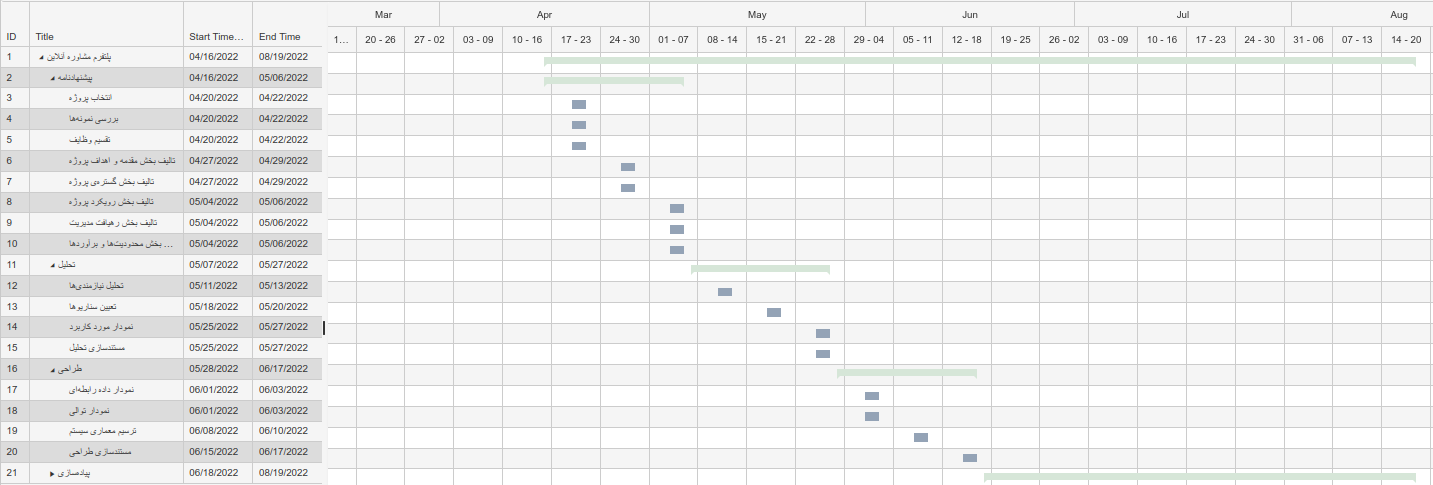
\includegraphics[width=1\textwidth]{Images/Gantt_1.png}
\newline
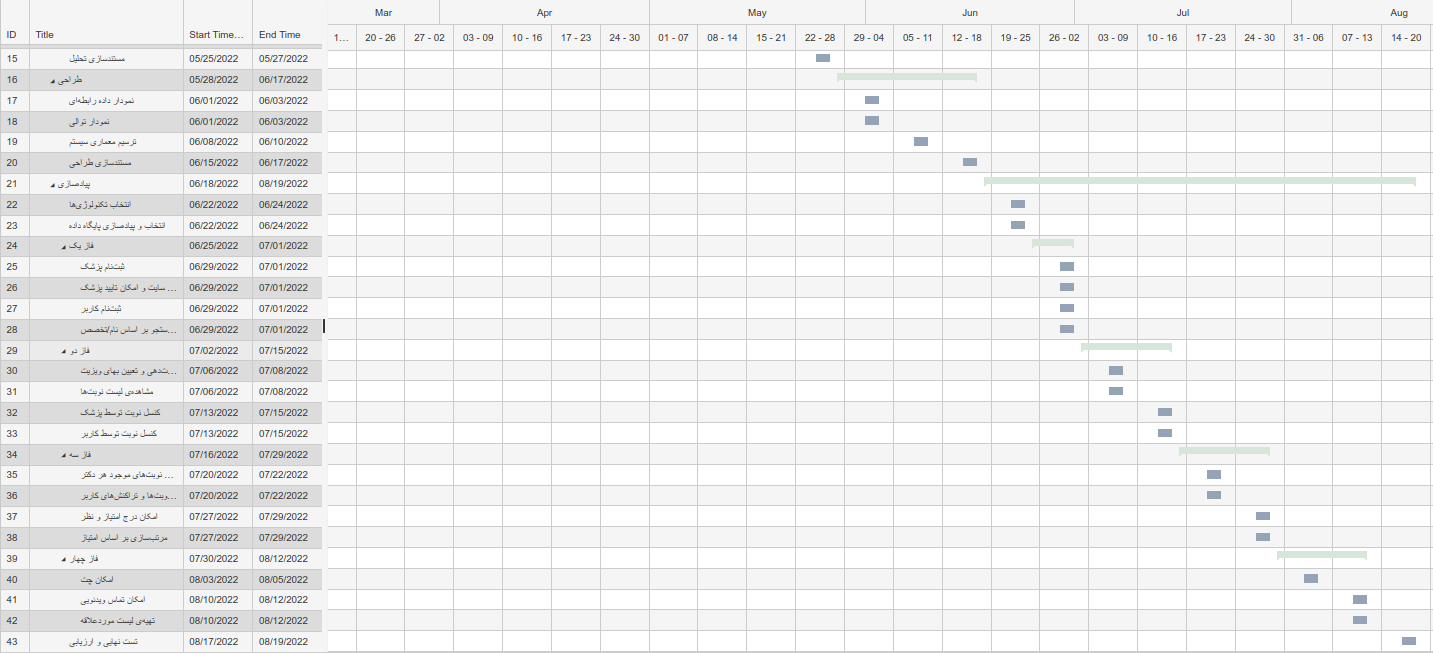
\includegraphics[width=1\textwidth]{Images/Gantt_2.png}

\subsubsection{برآورد مالی}
دستمزدها با توجه به شرایط مالی این حوزه و تجربه‌ی افراد به صورت زیر خواهد بود
\begin{itemize}
    \item یاشار ظروفچی - ساعتی ۲۸۰ هزار تومان معادل ۱۰ دلار
    \item فرزام زهدی‌نسب - ساعتی ۲۵۲ هزار تومان معادل ۹ دلار
    \item علی بالا‌پور - ساعتی ۲۵۲ هزار تومان معادل ۹ دلار
\end{itemize}

\subsubsection{برآورد هزینه‌ها}


\begin{table}
\centering
\resizebox{10cm}{!}{
\begin{tabular}{|c|c|c|}
\hline
هزینه  & نام بخش                & ID \\ \hline
6048\$   & سامانه مشاوره‌ی آنلاین & ۱  \\ \hline
1008\$ & پیشنهادنامه            & ۲  \\ \hline
1008\$ & تحلیل                  & ۱۱ \\ \hline
1008\$ & طراحی                  & ۱۶ \\ \hline
3024\$   & پیاده‌سازی             & ۲۱ \\ \hline
\end{tabular}%
}
\end{table}


\subsection{شرایط رضایتمندی}
\subsubsection{معیار‌های موفقیت}
در این قسمت، معیار‌هایی را مشخص می‌کنیم که تعیین کننده‌ی این هستند که پروژه با موفقیت به اتمام رسیده یا خیر. کنترل و نظرات بر این موارد در مراحل مختلف پروژه، به عهده‌ی مدیر پروژه است که می‌توان به موارد زیر اشاره کرد
\begin{enumerate}
    \item برخورداری از کیفیت مناسب
    \item اتمام پروژه در زمان مقرر
    \item اتمام پروژه با بودجه‌ی مشخص
\end{enumerate}
\subsubsection{پیش‌فرض‌ها}
تعدای از پیش‌فرض‌های پروژه در اینجا ذکر شده‌اند
\begin{itemize}
    \item کارجویان همگی دانشجوی دانشگاه صنعتی شریف هستند
    \item اطلاعات واردشده توسط کاربران معتبر هستند
    \item ادمین وبسایت به اطلاعات کاربران دسترسی خواهد داشت
    \item فعال بودن این سامانه از لحاظ حقوقی بلامانع است
\end{itemize}
\subsubsection{ریسک‌ها}
\begin{itemize}
    \item تغییر خواسته‌های کارفرما، که به تغییر برنامه‌ی زمانی یا ملی منجر خواهد شد
    \item کناره‌گیری یکی از اعضای تیم
    \item رونمایی از سامانه‌ی رقیب
\end{itemize}


\newpage

\medskip


% \bibliographystyle{unsrt-fa}
% \bibliography{mybibliography}




\end{document}

